\clearpage\mbox{}

\cxset{style51/.style={
 name=CHAPTER,
 numbering=WORDS,
 number font-size=Large,
 number font-weight=bold,
 number before={},
 number dot=,
 number position=rightname,
 chapter color=black!80,
 chapter font-size= Large,
 chapter font-weight= \bfseries,
 chapter before=\hspace*{0.9cm},
 number after=,
 chapter after=\vskip20pt,
 number color=black!80,
 title font-family=\normalfont,
 title font-color=black!80,
 title font-weight=,
 title font-size=\huge,
 title before=,
 title after=,
 title beforeskip=\hspace*{1cm}\minipage{10cm}\raggedright,
 title afterskip=\endminipage\par\vspace*{2cm},
 author block=false,
 epigraph width=\dimexpr(\textwidth-1cm)\relax,
 epigraph align=left,
 section font-weight=\normalfont,
 header style=empty}}

\cxset{style51}

\chapter{Introduction to Chapter Style\\ Fifty One}

\epigraph{\textbf{\sffamily Tuesday, October 16, 11:50 \textsc{a.m}, Cabinet Room}\par
               ``How do you know this is a medium-range ballistic missile?''}{President John F. Kennedy}


This is an unusual book with a rather unique style. The vertical rule is simple and breaks the monotony of a book that is heavy on text.
\begin{figure}[ht]
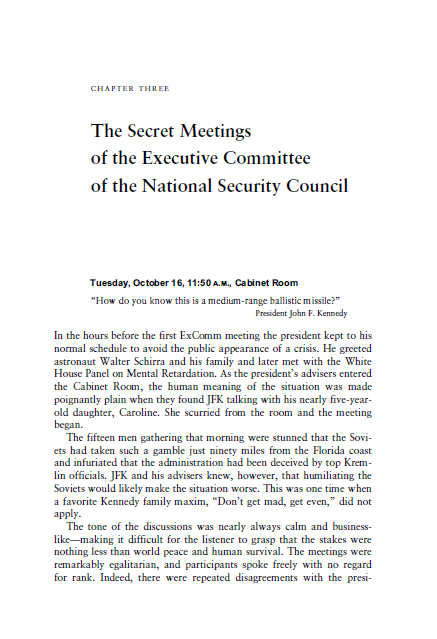
\includegraphics[width=0.48\textwidth]{./chapters/chapter51}\hfill
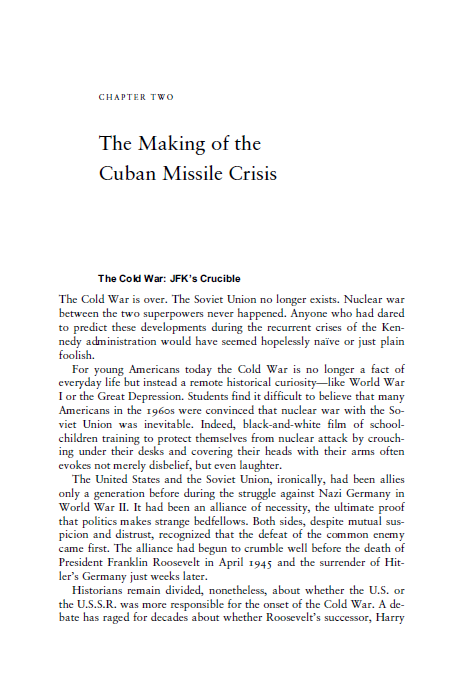
\includegraphics[width=0.48\textwidth]{./chapters/chapter51a}
\caption{Style 50 from the Oxford Handbook of Cuneiform Culture.}
\end{figure}

\section{Some notes}

If you observe this style carefully you will notice that the full title block, including the epigraph are set in from the left margin. This is achieved by setting appropriate \cs{hspace} lengths. The epigraph key width, needs to have the right distance and calculate the width. Example~ \ref{ch:style51} demonstrates the technique.

\begin{texexample}{Example setting-in the title block and epigraph}{ch:style51}
\cxset{style51,
   chapter opening=anywhere,
   epigraph align=right,
   epigraph width=\dimexpr(\textwidth-1.0cm)\relax,
  }
\chapter{Introduction to Chapter Style 51}
\epigraph{\textbf{\sffamily Tuesday, October 16, 11:50 \textsc{a.m}, Cabinet Room}\par
               ``How do you know this is a medium-range ballistic missile?''}{President John F. Kennedy}
\lorem
\end{texexample}

